\documentclass{article}

% set font encoding for PDFLaTeX, XeLaTeX, or LuaTeX
\usepackage{ifxetex,ifluatex}
\newif\ifxetexorluatex
\ifxetex
  \xetexorluatextrue
\else
  \ifluatex
    \xetexorluatextrue
  \else
    \xetexorluatexfalse
  \fi
\fi

\ifxetexorluatex
  \usepackage{fontspec}
\else
  \usepackage[T1]{fontenc}
  \usepackage[utf8]{inputenc}
  \usepackage{lmodern}
\fi
\usepackage{graphicx}
% used in maketitle
\title{Actividad 8}
\author{Jesús Adrián Zatarain Alvarado}

% Enable SageTeX to run SageMath code right inside this LaTeX file.
% documentation: http://mirrors.ctan.org/macros/latex/contrib/sagetex/sagetexpackage.pdf
% \usepackage{sagetex}

\begin{document}
\maketitle

\section{Introducción}

En sistemas dinámicos, el oscilador de van der Pol es un oscilador con amortiguamiento no lineal. Su evolución temporal obedece a una ecuación diferencial de segundo orden:
\\
\\
\begin{center}
{\displaystyle {d^{2}x \over dt^{2}}-\mu (1-x^{2}){dx \over dt}+x=0} 
\\
\\
{\displaystyle {d^{2}x \over dt^{2}}-\mu (1-x^{2}){dx \over dt}+x=0}
\\
\\
\end{center}
en la que x es la posición, función del tiempo t, y μ es un parámetro escalar que gobierna la no linealidad y el amortiguamiento.

El oscilador de Van der Pol es un sistema dinámico que incluye retroalimentación positiva
y un elemento resistivo no lineal. En su aplicación original, a principios del siglo
pasado, el oscilador eléctrico con un elemento no lineal se utilizó como precursor de los
primeros radios comerciales. Un circuito de este tipo favorece las oscilaciones pequeñas
y amortigua las grandes. En este artículo se analiza el comportamiento del oscilador de
Van der Pol con un voltaje x y un coeficiente de amortiguamiento k. Para k = 0 el sistema
es un oscilador lineal no amortiguado. A medida que épsilon crece, lo hace también la
no linealidad del sistema. El sistema tiene un solo punto de equilibrio, que es el punto
P(0,0), el cual siempre resulta ser inestable (repulsor), pero todas las trayectorias a partir
de él tienden en espiral a un ciclo límite y a éste también tienden a decaer aquellas trayectorias
cuyas amplitudes son más grandes que la amplitud del ciclo límite.

Balthasar Van der Pol fue un físico e ingeniero holandés que nació en Utrecht, en 1889 y murió en Wassenar en 1959. Aunque se conoce mejor a Van der Pol por su trabajo con circuitos eléctricos, descubrió una amplia variedad de sistemas que
presentan oscilaciones: el arpa eólica, un martillo neumático, el rechinido de un cuchillo en un plato, el ondear de una bandera al viento, el ocasional zumbido de una llave de agua, la recurrencia periódica de epidemias y crisis económicas… y,
por último, el latido del corazón. Van der Pol agrupó varios fenómenos en una sola categoría de sistemas que presentan oscilaciones periódicas.
\\
\\
En esta actividad se llevará a cabo la realización de lo mencionado en el oscilador de Van Der Pol.

\section{Modelo de Van der Pol}

El oscilador de Van der Pol modela un circuito eléctrico apareció en su artículo
“Relaxation-Oscillations”, publicado en la revista Philosophical Magazine en 1926, con particularidad es el uso de tubos de vacíos, estos actúan como una resistencia normal cuando la corriente es elevada, y como una resistencia “negativa” cuando la corriente es baja.

El oscilador de Van der Pol es un oscilador característico
de los sistemas oscilatorios no lineales, ya que éste presenta
un comportamiento auto-sostenible, es decir, un comportamiento
que lo lleva a siempre a una órbita periódica
atractora, esto es importante ya que los osciladores biológicos
como el marcapasos cardiaco (Nodo sinoatrial) que
genera por si solo una oscilación, que se dice autosostenida
por que al aplicarle ruido o condiciones iniciales fuera de
la órbita periódica, el sistema se dirige a ´esta por ser estable.
El sistema de ecuaciones ligado a este oscilador esta dado
por las ecuaciones de Lienard.

\section{Exploración de las soluciones del modelo en el Espacio Fase}

El teorema de Liénard prueba que el sistema tiene un ciclo límite. Aplicando la transformación de Liénard , donde el '.' indica derivada, la ecuación se puede escribir en forma bidimensional:
\\
\\
\begin{center}
{\displaystyle {\dot {x}}=\mu \left(x-{\frac {1}{3}}x^{3}-y\right)} {\displaystyle {\dot {x}}=\mu \left(x-{\frac {1}{3}}x^{3}-y\right)}
{\displaystyle {\dot {y}}={\frac {1}{\mu }}x.} {\displaystyle {\dot {y}}={\frac {1}{\mu }}x.}

\end{center}
\\
\\
Hay dos regímenes de funcionamiento interesantes para el oscilador no forzado:

Cuando μ = 0, no hay amortiguamiento, y la ecuación queda:
\\
\\
\begin{center}
{\displaystyle {d^{2}x \over dt^{2}}+x=0.} {\displaystyle {d^{2}x \over dt^{2}}+x=0.}
\end{center}
\\
\\
Es la fórmula del oscilador armónico simple sin pérdida de energía.
Cuando u > 0, el sistema alcanzará un ciclo límite, en el que se conservará la energía. Cerca del origen x = dx/dt = 0 el sistema es inestable, y lejos del origen hay amortiguamiento.
\\
\\
Utilizando una fuente de excitación sinusoidal Asin(wt) la ecuación diferencial queda:
\\
\\
\begin{center}
{\displaystyle {d^{2}x \over dt^{2}}-\mu (1-x^{2}){dx \over dt}+x-A\sin(\omega t)=0,}
\\
\\
\\
{\displaystyle {d^{2}x \over dt^{2}}-\mu (1-x^{2}){dx \over dt}+x-A\sin(\omega t)=0,}
\end{center}
\\
\\
en la que A es la amplitud de la ecuación de onda y ω su velocidad angular.

\section{Resultados y discusión}
Para esta práctica se utilizó parte del código de las actividades anteriores. Primeramente se importan las bibliotecas a utilizar, para pasar a definir la ecuación del oscilador de Van Der Pol. En seguida se especifican los valores de las variables a utilizar para generar los datos a graficar a continuación. Se generaran cuatro archivos con algunas cantidades parecidas pero diferiran en las condiciones iniciales.

Para el primero se toma como referencia la imagen proporcionada por la Web para saber las condiciones iniciales a la que están expuestos las cuatro gráficas.

\begin{verbatim}
from scipy.integrate import odeint 
from scipy import array, arange, pi, sin
import matplotlib.pyplot as plt
%matplotlib inline
from pylab import figure, plot, xlabel, grid, hold, legend, title, savefig, ylabel

def Van(X,t):
    x = X[0]
    x_point = X[1]
    dx = x_point
    dx_point = u*(1 - x*x)*dx - x
    return array([dx, dx_point])

#Parameters: 
t0 = 0
tmax = 50
pastemps = 0.05
time = arange(t0, tmax, pastemps)
x0 = -2.0
y0 = 4.0
u = 1.60

x, x_point = odeint(Van,(x0,y0),time).T

with open('dat1.dat', 'w') as f:
    for time, x, x_point in zip(time, x, x_point):
        print (time, x, x_point, file=f)
        
\end{verbatim}

Ya hechos los cuatro archivos con sus correspondientes datos, se pasa a graficar con ayuda de Python, los planos de fase del oscilador de Van der Pol no forzado.

El código utilizado está anexado a continuación.

\begin{verbatim}
import numpy as np
from numpy import loadtxt
from pylab import figure, plot, xlabel, grid, hold, legend, title, savefig, ylabel
from matplotlib.font_manager import FontProperties
import matplotlib.pyplot as plt
import matplotlib.colors as colors
%matplotlib inline

p2 = plt.figure(figsize=(8,6))
t0, x, x_point = loadtxt('dat1.dat', unpack=True)
figure(1, figsize=(6, 4.5))
plt.xlabel('$x$', fontsize = 20)
plt.ylabel('$\dot{x}$', fontsize = 20)
plt.plot(x, x_point, 'blue')
title('Phase portrait')

t0, x, x_point = loadtxt('dat2.dat', unpack=True)
plt.plot(x, x_point, 'blue')


t0, x, x_point = loadtxt('dat3.dat', unpack=True)
plt.plot(x, x_point, 'blue')


t0, x, x_point = loadtxt('dat4.dat', unpack=True)
plt.plot(x, x_point, 'blue')


t0, x, x_point = loadtxt('dat1.dat', unpack=True, skiprows=250)
plt.plot(x, x_point, 'red')

savefig('phasePortrait.png', dpi=100)

\end{verbatim}

que resulta en la siguiente imagen:

\begin{center}
    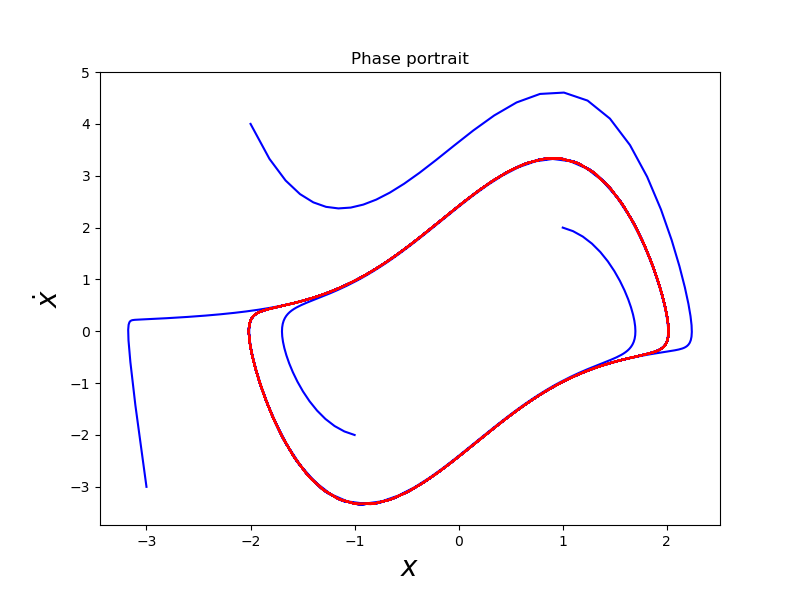
\includegraphics[width=6cm, height=6cm]{Van1.png}
\end{center}

Lo siguiente es realizar la evolución del ciclo límite en el plano fase. Se hace al variar continuamente el parámetro u, obteniendo así la siguiente imagen.

\begin{center}
    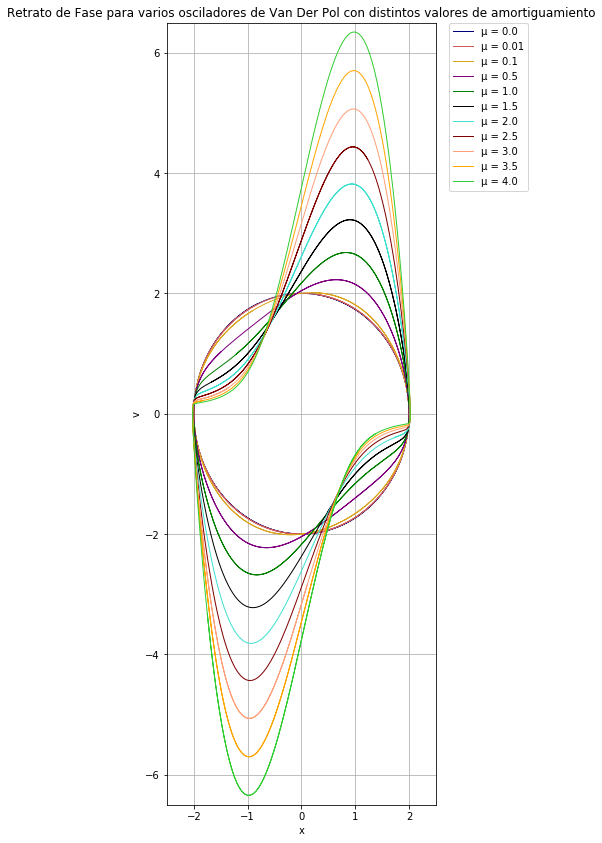
\includegraphics[width=6cm, height=6cm]{Van2.png}
\end{center}

Ahora se realizará el oscilador en dos maneras, uno no forzado y el otro forzado ; donde en el primero u=0 y en el otro se tiene que hay una fuente de exitación sinuidal. Ambos quedan de la siguiente forma.

\begin{center}
    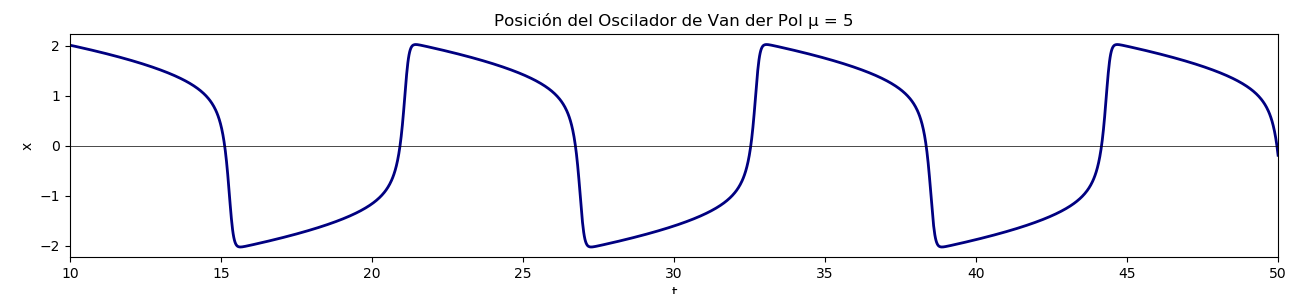
\includegraphics[width=6cm, height=6cm]{Van3.png}
\end{center}

\begin{center}
    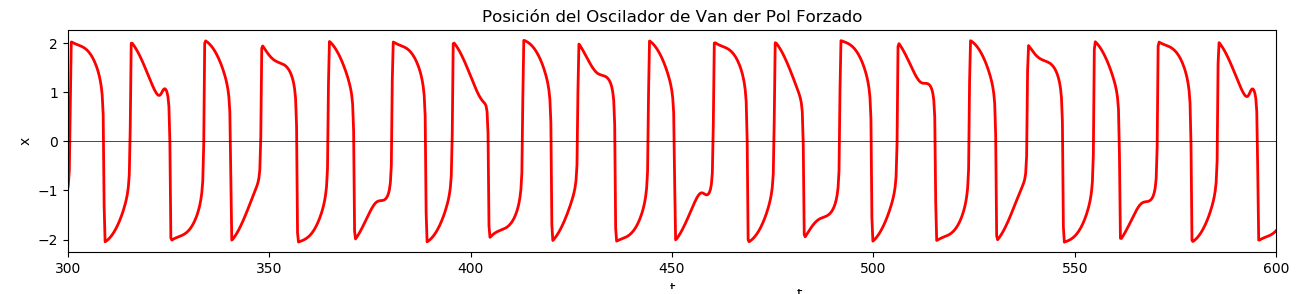
\includegraphics[width=6cm, height=6cm]{Van4.png}
\end{center}

\begin{center}
    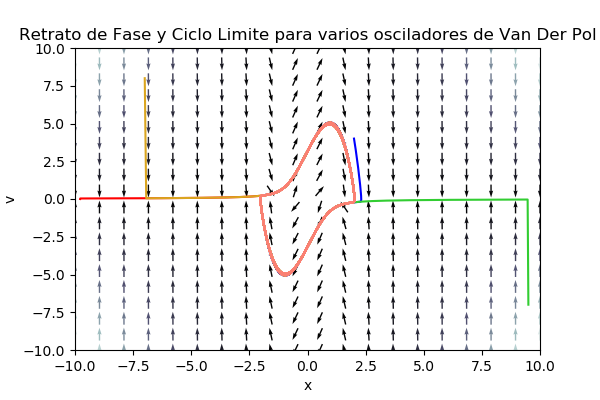
\includegraphics[width=6cm, height=6cm]{Van5.png}
\end{center}

\section{Bibliografía empleada}
https://en.wikipedia.org/wiki/Van_der_Pol_oscillator
\\
\\
https://es.wikipedia.org/wiki/Oscilador_de_van_der_Pol
\\
\\
https://www.uab.edu/medicine/id/.../93-barbara-van-der-pol


\section{Apéndice}

1.- Este ejercicio pareciera similar al desarrollado en las actividades 6 y 7. ¿Qué aprendiste nuevo?
\\
\\
A cómo acomodar distintos datos en una sola gráfica y trasformar ecuaciones diferenciales
\\
\\
2.- ¿Qué fue lo que más te llamó la atención del oscilador de Van der Pol?
\\
\\
La sencillez aparente con la que es descrito y su utilidad en los circuitos eléctricos.
\\
\\
3.- Has escuchado ya hablar de caos. ¿Por qué sería importante estudiar este oscilador?
\\
\\
Debido a que está descrito por ecuaciones no lineales
\\
\\
4.- ¿Qué mejorarías en esta actividad?
\\
\\
Añadiría un poco más acerca de este oscilador
\\
\\
5.- ¿Algún comentario adicional antes de dejar de trabajar en Jupyter con Python?
\\
\\
Es un entorno muy amigable que lo seguiré usando para proyectos más adelante en la carrera.
\\
\\
6.- Cerramos la parte de trabajo con Python ¿Que te ha parecido?
Muy buena experiencia y muy útil para la carrera de física.
\end{document}
